% !Mode:: "TeX:UTF-8"
% !TEX program  = xelatex

%\documentclass{cumcmthesis}
\documentclass[withoutpreface,bwprint]{cumcmthesis} %去掉封面与编号页
%\usepackage{ctex}    
%用了第一行的documentclass里已经包含了大部分数学公式需要的宏包,不需要再引入了
%\renewcommand\theenumi{(\roman{enumi})} 
%\renewcommand\labelenumi{\theenumi}

\title{高压油管的压力控制模型研究}
\tihao{A}
\baominghao{201919029020}
\schoolname{南方科技大学}
\membera{熊卓晨}
\memberb{邓钧泽}
\memberc{孔祥喆}
\supervisor{李景治老师}
\yearinput{2019}
\monthinput{09}
\dayinput{12}

\begin{document}
\maketitle

 \begin{abstract}
 	本文通过研究某高压燃油系统的工作原理,探究燃油泵入和喷出的间歇性工作机制对高压油管内燃油压强的变化和控制的影响,得到了燃油在不同条件下泵入和喷出的实际工作情况模型。问题中多次出现的维持压强的问题,由于压强是和密度相关的,在体积一定的情况下,要使高压油管内压强尽量稳定的问题,实质上可以理解为在一段比较长的时间内使得燃油进入质量量与喷出质量相等。
 	
 	对于问题一,燃油的进入和喷出都呈周期性变化,虽然进入和喷出的周期不同,但是我们可以将参考的那段时间尽可能选的长,这样维持压强不变也可以理解为单位时间内的流入、喷出质量相等。实际上,随时间的变化过程中管内燃油的质量会有增减的波动,不是严格的稳定。我们忽略这种波动,在该前提下,通过$\triangle M_{\text{入}}=\triangle M{\text{出}}$的等量关系建立方程,根据不同压强条件下燃油密度的变化可以解出单向阀每次应开启的时长。至于如何将管内的压强从100MPa增加到150MPa,实质时一定时间内,管内燃油质量的增加。由于管内燃油的压强随时间的变化而变化,从而影响燃油进入的速率以及喷出的密度,我们需要建立燃油进入的速率和喷出密度分别对时间的函数,进而确立模型求解。
 	
 	对于问题二,根据附件1作出凸轮边缘的曲线与角度的图像,建立凸轮运动的模型,可模拟高压油泵的工作原理,进而近似计算出凸轮运动一个周期,泵入油管的燃油质量。再根据一个喷油周期内针阀升程与时间的关系,模拟针阀的升程关于时间的函数,得出一个周期内喷孔出油体积的情况,要注意的是,根据针阀限制流量的远离,针阀升程到达一定数值时,针阀可以视为“完全开启”,针阀不完全开启时,需要使用附件2数据拟合升程关于时间的函数,计算出油有效速率对时间的函数,通过积分求得实际的出油体积。同样在这里假定油管内的燃油质量是严格恒定的,利用问题一的思路$\triangle M_{\text{入}}=\triangle M_{\text{出}}$的等量关系建立方程,解出入油量随时间变化的关系,从而确定凸轮的角速度。
 	
 	对于问题三,增加一个喷油孔之后,凸轮的转速会发生相应的增加,以维持管内燃油压强的不变。这个时候管内燃油的压强对于时间的函数其实不是严格恒定的,会有上下的波动。为了减小这种波动,我们需要将两个喷油孔的工作时间错开。而在增加了新的减压阀D之后,不妨从一个极端的情况,即一直将D阀开启,从该情况出发,分析凸轮转速,及D阀的影响。以该极限状况出发,向一般状况分析。
 		
 	\keywords{数据拟合\quad  数值分析\quad  \textsc{Matlab}图像处理}
 \end{abstract}

%目录
%\tableofcontents

%\newpage
\section{问题背景}
燃油进入和喷出高压油管是许多燃油发动机工作的基础,\cref{fig:youtube-picture} 给出了某高压
燃油系统的工作原理,燃油经过高压油泵从 A 处进入高压油管,再由喷口 B 喷
出。燃油进入和喷出的间歇性工作过程会导致高压油管内压力的变化,使得所喷
出的燃油量出现偏差,从而影响发动机的工作效率。

\begin{figure}[!h]
	\centering %图片全局居中
	%并排几个图,就要写几个minipage
	\begin{minipage}[b]{0.4\textwidth} %所有minipage宽度之和要小于1,否则会自动变成竖排
		\centering %图片局部居中
		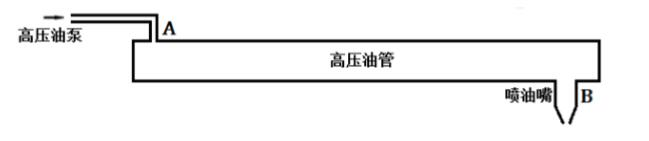
\includegraphics[width=1\textwidth]{youtube} %此时的图片宽度比例是相对于这个minipage的,不是全局
		\caption{高压油管示意图}
		\label{fig:youtube-picture}
	\end{minipage}
	\begin{minipage}[b]{0.4\textwidth} %所有minipage宽度之和要小于1,否则会自动变成竖排
		\centering %图片局部居中
		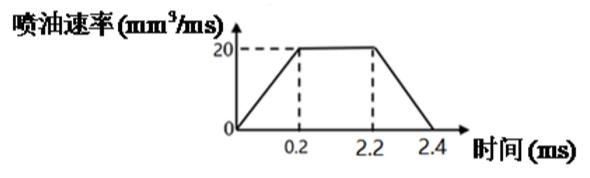
\includegraphics[width=1\textwidth]{penyousudu}%此时的图片宽度比例是相对于这个minipage的,不是全局
		\caption{喷油速率示意图}
		\label{fig:penyou-picture}
	\end{minipage}
\end{figure}
题目中某个高压油管的基本参数如下:

高压油管的内腔长度为 500mm,内直径为 10mm,供油入口
A 处小孔的直径为 1.4mm,通过单向阀开关控制供油时间的长短,单向阀每打开
一次后就要关闭 10ms。喷油器每秒工作 10 次,每次工作时喷油时间为 2.4ms,
喷油器工作时从喷油嘴 B 处向外喷油的速率如 \cref{fig:penyou-picture} 所示。高压油泵在入口 A 处提供的压力恒为 160 MPa,高压油管内的初始压力为 100 MPa。
\section{问题的提出}
\subsection{问题重述}
由题目给出的背景知识及三个问题可以分析出本文共需解决5个问题,通过解决这5个问题建立模型分析在高压油管中多个不同参数改变的情况下,如何调整油泵参数使发动机工作效率最大化。这些问题分别为:

\begin{enumerate}[label=\Roman*.]
	\item 要将高压油管内的压力尽可能稳定在 100 MPa 左右,如何设置单向阀每次开启的时长?\label{ques1} 
	\item 要将高压油管内的压力从 100 MPa 增加到 150 MPa,且分别经过约 2 s、5 s 和10 s 的调整过程后稳定在 150 MPa,单向阀开启的时长应如何调整? \label{ques2} 
	\begin{figure}[!h]
		\centering 
		\begin{minipage}[b]{0.6\textwidth} 
			\centering 
			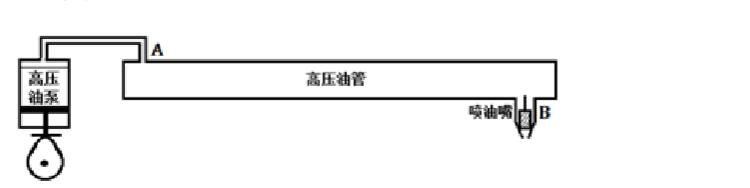
\includegraphics[width=1\textwidth]{realyoutube} 
			\caption{高压油管实际工作示意图}
			\label{fig:realyoutube-picture}
		\end{minipage}
		\begin{minipage}[b]{0.39\textwidth} 
			\centering 
			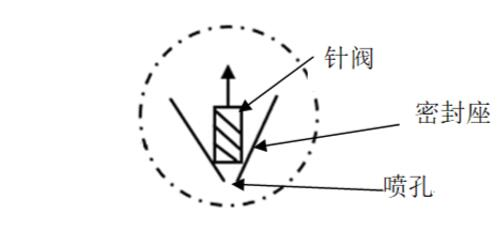
\includegraphics[width=1\textwidth]{muzzle}
			\caption{喷油器喷嘴示意图 }
			\label{fig:muzzle-picture}
		\end{minipage}
	\end{figure}
	\item 实际工作中,高压油管A处的燃油来自高压油泵的柱塞腔出口,喷油由喷油嘴的
	针阀控制。高压油泵柱塞的压油过程如\cref{fig:realyoutube-picture}所示,
	凸轮驱动柱塞上下运动。针阀的结构如\cref{fig:muzzle-picture}所示,
	燃油通过针阀的开闭喷出。在题目给出的基本参数条件下,
	确定凸轮的角速度,使得高压油管内的压力尽量稳定在100 MPa左右。\label{ques3} 
	
	\item 在上一问的基础上,再增加一个喷油嘴,每个喷嘴喷油规律相同,喷
	油和供油策略应如何调整?\label{ques4} 
	\begin{figure}[!h]
			\centering %图片局部居中
			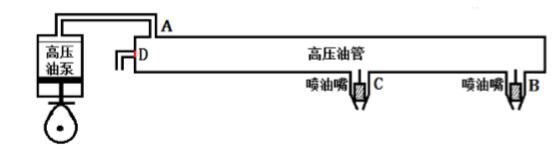
\includegraphics[width=0.8\textwidth]{doublemuzzle}
			\caption{具有减压阀和两个喷油嘴时高压油管示意图 }
			\label{fig:doublemuzzle-picture}
	\end{figure}

	\item 为了更有效地控制高压油管的压力,现计划在D处安
	装一个单向减压阀(\cref{fig:doublemuzzle-picture})。单向减压阀出口为直径为1.4mm的圆,打开后高压油
	管内的燃油可以在压力下回流到外部低压油路中,从而使得高压油管内燃油的压力减小。请给出高压油泵和减压阀的控制方案。 \label{ques5} 
\end{enumerate}
\subsection{问题分析}
\begin{enumerate}[label=\Roman*.]
	\item 根据题意,要尽可能维持高压油管内的压力为100Mpa,则单向阀门的入油质量和喷油嘴的出油质量应尽量维持在相等状态。由给出的公式可以求出不同压强条件下的燃油密度,再根据入油和出油的体积,建立方程式,解出维持100Mpa所需要的单向阀每次开启的时间。
	\item 如果要将燃油压强提升到150Mpa,其实质是高压油管中燃油质量的增加,先计算出燃油质量的增量,再建立相应方程式,解出单向阀每次开启的时间。其中,由于高压油管内的压强在时刻变化,需要做相应的近似处理。
	\item 该问题相对于前两题的变化是进油口和出油口都从某个理想状态更改为都在变化的情况。所以该题的解决方向是先根据已知数据模拟出进油和出油质量关于时间的变化情况,即可把问题转化为问题\ref{ques1}中的进、出高压油管的燃油质量相等问题,可以建立方程,从而求解。
	\item 该题在问题\ref{ques3}的基础上增加了一个喷油嘴。这个改变从抽象到公式中就是出油量发生了改变。而由于两个油嘴喷油规律相同,对喷油时间的调整方案就决定了对管内压强的影响大小。可猜测将喷油时间错开能够让每个时间段的压强波动尽可能小,然后计算出对应的油泵参数可以得出最佳策略。
	\item 此问题是一个较有开放性的题目,本小组认为可以先从一种极端情况:保持减压阀完全开启,来考虑压强的变化情况。然后把模型从特殊到一般情况进行推广,得到普遍状况下减压阀和凸轮的调整方案。
\end{enumerate}
\section{模型基本假设}
\begin{enumerate}
	\item 该品种燃油在题目中的温度和压强下不会被压燃。
	\item 假设该油管的形状体积严格符合数据,内壁没有凹凸及误差。
	\item 模型一的背景下高压油泵的出口压强保持恒定。
	\item 模型一的特例中油管内的轻微压强变化可忽略。
	\item 模型二中喷油嘴的针阀与油泵的柱塞只做上下平移没有受扰动便宜。
\end{enumerate}
\section{符号说明}
\begin{center}
	\begin{tabular}{cc|cc}
		\toprule
		\makebox[0.05\textwidth][c]{符号}	&  \makebox[0.2\textwidth][c]{意义}  & \makebox[0.05\textwidth][c]{符号}	&  \makebox[0.2\textwidth][c]{意义} \\
		\midrule
		$V_{0}$	  & 高压油管容积($mm^{3}$)                        & 
		$C$       & 流量系数                                     \\
		$A$       & 油泵出油口面积($mm^{2}$)                   &
		$h$       & 柱塞上下支点距离($mm$)                            \\
		$A_{\text{内}}$ & 柱塞腔内面积($mm^{2}$)           &
		$h_{0}$   & 柱塞上升高度($mm$)                          \\
		$A_{t}$       & t时刻油嘴喷油面积($mm^{2}$)           &
		$Q_{0}$   & 初始压强燃油流入速率($mm^{3}/ms$)              \\
		$A_{\text{孔}}$       & 喷油嘴喷孔面积($mm^{2}$)            & 
		$Q_{t}$   & t时刻燃油流入速率($mm^{3}/ms$)                  \\
		$t_{0}$   & 油管达到目标压强时间($ms$)                  &
		$Q_{c}$   & 每周期内喷嘴喷油量($mm^{3}/100ms$)           \\
		$t_{x}$   & 单向阀开启的时间($ms$)                          &
		$\overline{Q_{\lambda}}$    & 等效流入速率($mm^{3}/ms$)     \\
		$\rho_{xMPa}$   & $xMPa$下燃油密度($mg/mm^{3}$)       &
		$P_{t}$   & t时刻油管内的燃油压强($MPa$)                 \\
		$\rho_{0}$   & 初始压强对应密度($mg/mm^{3}$)                &
		$P_{0}$   & 初始时刻油管燃油压强($MPa$)                  \\
		$\rho_{\text{低压}}$   & 低压燃油密度($mg/mm^{3}$)           &
		$V_{\text{剩}}$   & 油泵剩余燃油体积($mm^{3}$)                  \\
		$\overline{\rho_{c}}$   & 等效流出密度($mg/mm^{3}$)         &
		${\triangle M}$   & 始末时刻油管内燃油质量差($mg$)           \\
		$s_{t}$   & t时刻针阀的升程($mm$)                            &
		${\triangle M_{\text{增}}}$   & 凸轮转动一圈油管燃油增量($mg$)                     \\
		${T_{\text{轮}}}$   & 凸轮旋转周期($ms$)                     &
		${\triangle M_{\text{减}}}$   & $100ms$内油管燃油减少量($mg$)                     \\	
		\bottomrule
	\end{tabular}
\end{center}
\section{模型的构建与求解}
\subsection{维持油管恒压的单向阀开启时间模型}\label{model1}
根据题意,油泵的压强是理想情况下可以维持恒定的,只需要考虑出油和进油对高压油管部分的压强影响。因为压强这个数值不好处理,我们需要把这个物理量处理为质量。根据公式$\frac{E}{\rho} = \frac{\triangle P}{\triangle \rho}$可以得知油管内燃油密度和压强的联系,从而计算出$160MPa$下的密度。
\subsubsection{模型特例:高压油管内压强始终保持恒定}\label{case0}
在第一个小问题的假设下,可以把高压油管内部的燃油密度近似为定值。维持压强的问题就可以等价于进油口进油速率等于出油口出油速率。据此,可以得到以下方程
\begin{equation}
	\frac{ \rho_{160MPa}\times Q_{0}\times t_{x}}{t_{x}+10}=\frac{ \rho_{100MPa}\times Q_{c}}{100}\label{eq:ques1}
\end{equation}

其中,方程中的一些重要物理量 \footnote{如$Q_{c}$ , $t_{x}$,$A$等可以由题面数据直接得到或通过简单计算式得到的中间变量在此不列出} 由以下计算式解出:
\begin{equation*}
Q_{0} = C\times A\times \sqrt{\frac{2\times (160-100)}{\rho_{160MPa}}}\label{eq:ques1-1}
\end{equation*}

%对公式$\frac{E}{\rho} = \frac{\triangle P}{\triangle \rho}$移项积分可以得到
\begin{equation*}
	\int_{}^{}{\text{d}P} = \int_{}^{} \frac{E}{\rho}{\text{d}\rho}\label{eq:ques1-2}
\end{equation*}

代入$100MPa$时的数据可以得到,
\begin{equation}
P_{t} = E\ln\rho+452.9\label{eq:ques1-3}
\end{equation}



解出方程\cref{eq:ques1}得到时间$t_{x} = 0.2747ms$,该解即为问题\ref{ques1}的答案

\subsubsection{推广模型:压强发生改变后维持最终压强的单向阀开启时间模型}\label{case1}
高压油管压强在输油过程中发生改变会导致高压油泵的输入速率和喷嘴的输出密度变化,因此不再适用于特例情况下的单向阀开启时间模型。随着高压油管内压强的变大,输入速率逐渐变小而输出的密度在不断增大,``压强-时间''函数在达到稳定状态前可近似拟合 为一个$\ln x$型的函数\footnote{该结果根据附件3中的数据近似拟合得到},即以下形式:
\begin{equation}
	P_{t} = 100+\lambda\ln (t+1)\label{eq:ques2}	
\end{equation}

其中$t$为达到稳定前的自变量时间,$\lambda$为$t_{0}$时间到达稳定状态所对应的一个常数。在题面给出$t_{0}=2000ms$,$t_{0}=5000ms$,$t_{0}=10000s$的情况下,可以计算出他们相对应的$\lambda$值,然后利用\textsc{Matlab}绘制了下图,可近似看作高压油管内气体压强随时间变化的曲线。

\begin{figure}[!h]
	\centering 
	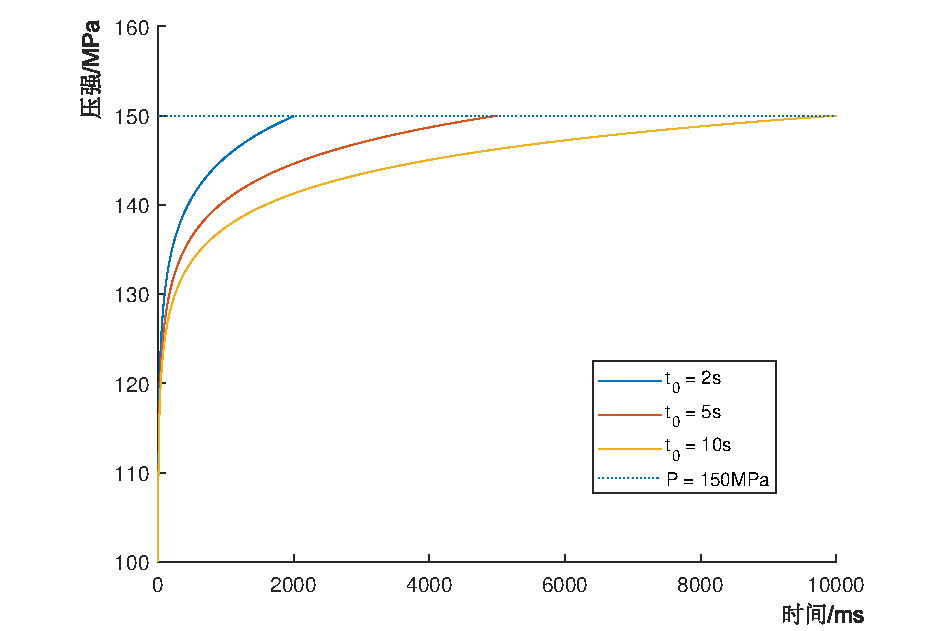
\includegraphics[width=0.8\textwidth]{P-tfigure}
	\caption{高压油管内气体压强随时间变化曲线}
	\label{fig:f(t)-picture}
\end{figure}
\newpage
首先,末态和初态的压强差,可以转化为质量的增加,那么高压油管内的压强从${100MPa}$增加为${150MPa}$,实质上是高压油管内燃油的质量增加${\triangle M}$,根据质量与密度和体积的关系,很容易计算出增量${\triangle M}$。
由于高压油管内的压强变化快,难以用模拟函数某一点的值近似表示该时刻的管内油压。所以用积分的平均值,来表示流入、流出油管的有效平均值,将变化的流入速率和变化的流出燃油密度,用其对应的有效平均值来近似等效。此时高压油泵的输入速率和喷嘴的输出密度都为恒定值,在$t_{0}$时间内,可以用$t$表示随着时间高压油管内燃油质量的增量,如果可以解出某个$t_{x}$值可以使其增量为${\triangle M}$,那么这个值即为所求单向阀开启时间。
\subsubsection{多种情况下该模型的求解}
根据上述对模型的描述,我们可以将模型抽象为以下三个等式:
\begin{enumerate}
	\item 等效平均流入速度的等式
	\begin{equation*}
	\overline{Q}_{\lambda} = \frac{1}{t_{0}}\times \int_{0}^{t_{0}} C\times A\times \sqrt{\frac{2\times (160-P_{t})}{P_{160MPa}}}{\text{d}t}\label{eq:ques2-1}	
	\end{equation*}
	\item 等效平均流出密度的等式\footnote{该等式中的常数由计算式\cref{eq:ques1-3}得到}
	\begin{equation*}
	\overline{\rho_{c}} = \frac{1}{t_{0}}\times \int_{0}^{t_{0}} e^{\frac{P_{t}-452.9}{E}}{\text{d}t}\label{eq:ques2-2}	
	\end{equation*}
	\item 该模型的求解方程
	\begin{equation}
	t_{0}\times(\frac{\overline{Q_{\lambda}}\times t_{x}}{t_{x}+10}\times \rho_{160MPa}-\frac{Q_{c}}{100}\times \overline{\rho_{c}})-\triangle M = 0\label{eq:ques2-3}	
	\end{equation}
	使用\textsc{Matlab}解出方程\cref{eq:ques2-3},所得到的解即是我们所需要求的阀门开启时间。以下分别就$t_{0}$的几种取值讨论解的结果。
\end{enumerate}
\paragraph{$t_{0}=2000ms$时}~{}

代入函数\cref{eq:ques2}可计算出$\lambda=6.57$,运用该值解方程\cref{eq:ques2-3},解得$t_{x} =2.7511$。该值即为调整时间内单次开启单向阀的时长。

\paragraph{$t_{0}=5000ms$时}~{}

代入函数\cref{eq:ques2}可计算出$\lambda=5.87$,运用该值解方程\cref{eq:ques2-3},解得$t_{x} = 1.5160ms$。该值即为调整时间内单次开启单向阀的时长。
\paragraph{$t_{0}=10000ms$时}~{}

代入函数\cref{eq:ques2}可计算出$\lambda=5.43$,运用该值解方程\cref{eq:ques2-3},解得$t_{x} = 1.1524ms$。该值即为调整时间内单次开启单向阀的时长。

\paragraph{压强达到$150MPa$时}~{}

当压强稳定在$150MPa$时,该模型又回到了特例的条件下,运用\ref{case0}的结论可以得到$t_{x} = 0.7383ms$。该值即为稳定后每次单向阀的开启时间

\subsubsection{结果分析}

综上,可以得到问题\ref{ques2}的结果
\begin{enumerate}
	\item $t_{0}=2000ms$时,应调整单项阀的开启时长为稳定前每次开启$1.5160ms$,稳定后每次开启$ 0.7383ms$。
	\item $t_{0}=5000ms$时,应调整单项阀的开启时长为稳定前每次开启$6.7607ms$,稳定后每次开启$1.3794ms$。
	\item$t_{0}=10000ms$时,应调整单项阀的开启时长为稳定前每次开启$2.7771ms$,稳定后每次开启$1.3794ms$。
\end{enumerate}
\subsection{维持高压油管压强的凸轮角速度模型}\label{model2}

\subsubsection{题目背景下油泵处的进油模型}\label{case2}
首先根据附件1提供的数据,利用\textsc{matlab}在极坐标下作出了凸轮边缘曲线图像。\footnote{绘图源代码详见附件}。

\begin{figure}[!h]
	\centering 
	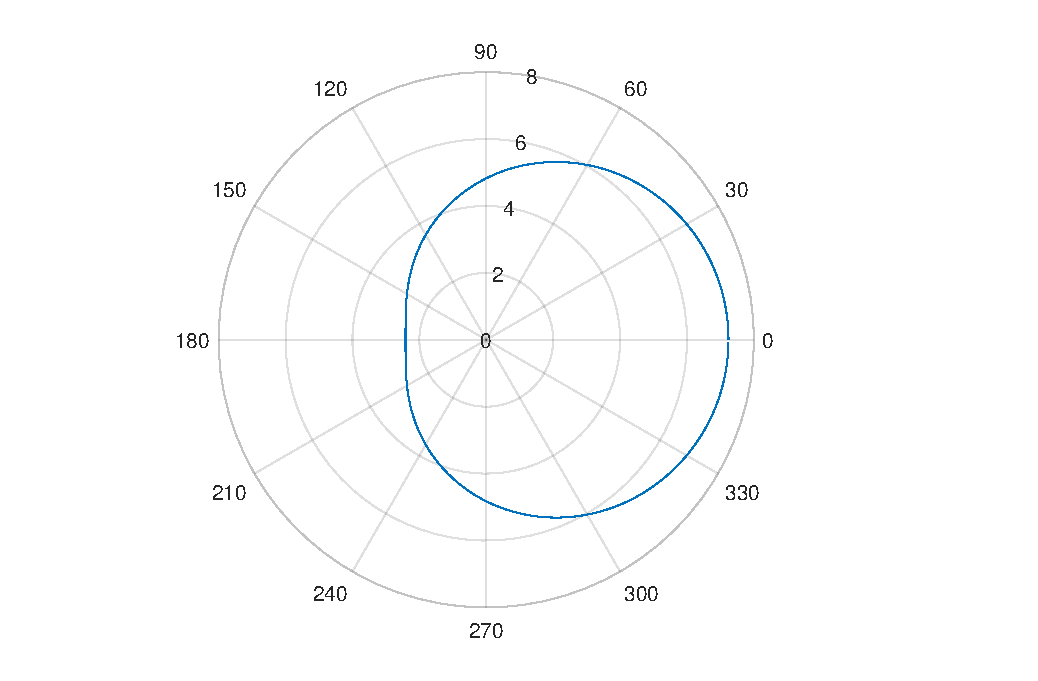
\includegraphics[width=0.8\textwidth]{tulun}
	\caption{凸轮轮廓示意图}
	\label{fig:tulun-picture}
\end{figure}

如\cref{fig:tulun-picture}所示,蓝色曲线为凸轮轮廓,凸轮绕极点旋转。

分析可知,极径最大值与最小值的差即为柱塞运动到上、下止点的距离,记为h。根据克拉伯龙方程,以及附件1的数据可以近似求出凸轮在某一角度时,即可刚好打开单向阀门。 当凸轮继续运动到某一位置时,高压油泵内的压强下降到100MPa,单向阀门关闭。在这个过程中,一定质量的燃油被压进高压油管。把该过程用函数表达出来则为下式。

\begin{equation}
\triangle M_{\text{增}}= M_{\text{初}}-M_{\text{末}}\label{eq:ques3-5}
\end{equation}

其中,$M_{\text{初}}$为阀门开启前油泵内的燃油质量,可以由下式算出,
\begin{equation*}
M_{\text{初}} = \rho_{\text{低}}\cdot (V_{\text{剩}}+\pi r^{2}_{\text{内}}\cdot h)\label{eq:ques3-6}
\end{equation*}

$M_{\text{末}}$为阀门关闭后油泵内的燃油剩余的质量,可以由下式算出,
\begin{equation*}
M_{\text{末}} = \rho_{100MPa}\cdot V_{\text{剩}}\label{eq:ques3-7}
\end{equation*}

\subsubsection{题目背景下喷油嘴的喷射模型}\label{case3}
喷油嘴通过针阀来控制喷油速率,其原理是当针阀升程为正时,针阀底端与密封座相应截面形成一个圆环:如果该圆环面积小于喷孔面积,则喷油速率取决于圆环面积大小;如果圆环面积大于喷孔面积,此时无论针阀的升程能否继续增大,喷油速率只取决于喷孔面积大小。通过以上分析,及附件2,拟合出每个周期内喷油速率随时间变化的函数及图像。

\begin{figure}[!h]
	\centering 
	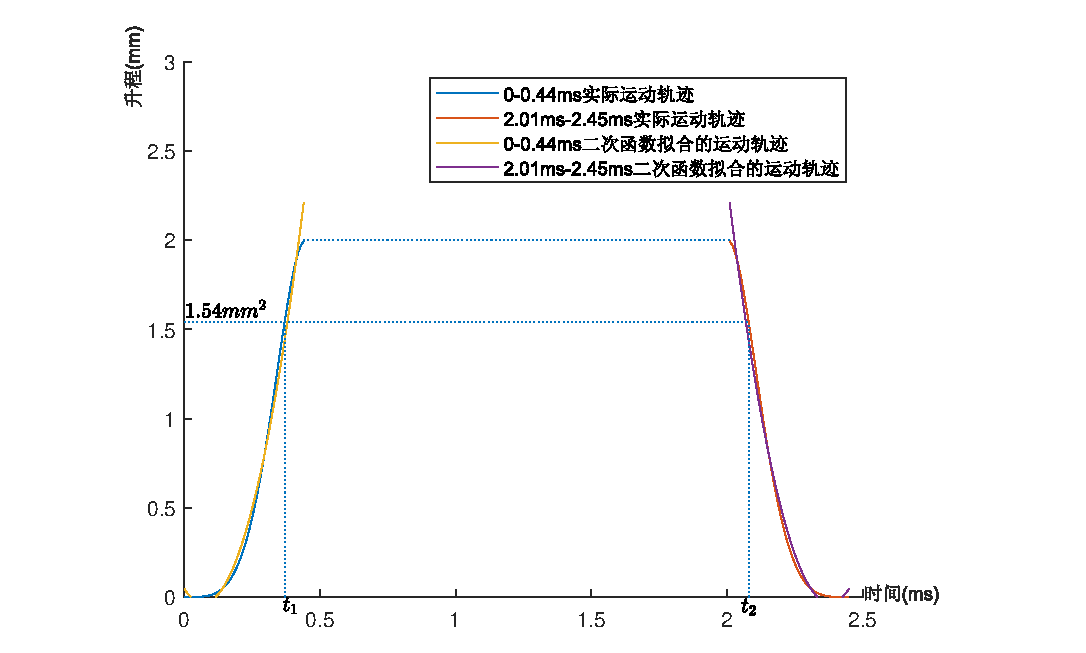
\includegraphics[width=0.8\textwidth]{zhenfa}
	\caption{针阀升程随时间变化的拟合图像}
	\label{fig:Q(t)-picture}
\end{figure}

从图片可以看出,在$t_{1}-t_{2}$区间内圆环面积大于喷油孔的面积,因此这段时间的出油速率由喷油孔截面积决定。而在$0-t_{1}$及$t_{2}-t_{\text{末}}$的时间内出油速率则与该时刻圆环的面积$A_{t}$有关,喷油嘴的出油效率$Q_{c}$可以由下述分段函数表示,其中$t_{\text{末}} = 2.45ms$
\begin{equation}
Q_{c}(t) =
\begin{cases}
C\times A_{\text{孔}}\times \sqrt{\frac{2\times \triangle P}{\rho_{100MPa}}} &   t_{1}<t<t_{2} ,\\
C\times A_{\text{t}}\times \sqrt{\frac{2\times \triangle P}{\rho_{100MPa}}} &   0<t<t_{1},t_{2}<t<t_{\text{末}}
\end{cases}\label{eq:ques3-1}
\end{equation}

由圆环的面积计算公式可知,在$t_{1}-t_{2}$时间段内$A_{t}$由下述函数表示,
\begin{equation*}
A_{t} = \pi\times ((r_{1}+\triangle r)^{2}-r_{1}^{2})\label{eq:ques3-2}	
\end{equation*}

该式中的$\triangle r$为此时圆锥切面半径与针阀半径的差值,由\cref{fig:muzzle-picture}和题面数据可知该值可以用下述函数表示,
\begin{equation*}
\triangle r = s_{t}\times\tan(9^{\circ})\label{eq:ques3-3}	
\end{equation*}
 
为了让高压油管内油压的变化量尽可能小,我们需要在尽可能短的周期内使油管进出的燃油质量相等。因此,我们需要在$0-t_{\text{末}}$这个周期内对函数式\cref{eq:ques3-1}进行积分得到这个小段时间内的出油量,记作$Q_{c}$,
\begin{equation}
Q_{c} = \int_{0}^{t_{1}}Q_{t}\text{d}x+\int_{t_{1}}^{t_{2}}Q_{\text{孔}}\text{d}x+\int_{t_{2}}^{t_{\text{末}}}Q_{t}\text{d}x \label{eq:ques3-4}	
\end{equation}

\subsubsection{求解高压油泵中凸轮的角速度}
结合\ref{case2}和\ref{case3}两个模型的结论,可以将维持压强的问题转化为在一段时间内进、出高压油管的燃油质量相等的问题。建立如下方程,

\begin{equation}
 \frac{\triangle M_{\text{增}}}{T_{\text{轮}}}=\frac{\left(\int_{0}^{t_{1}}Q_{t}\text{d}x+\int_{t_{1}}^{t_{2}}Q_{\text{孔}}\text{d}x+\int_{t_{2}}^{t_{\text{末}}}Q_{t}\text{d}x\right)\times \rho_{100MPa}}{100}\label{eq:ques3-10}	
\end{equation}

求解方程\cref{eq:ques3-10}可以得到凸轮旋转的周期$T_{\text{轮}} = 96.14ms$,由周期与转速的关系$\omega = \frac{2\pi}{T}$,可以得知$\omega = 0.0654 rad/ms$,该值即为问题\ref{ques3}所需求的凸轮角速度。
\subsection{增加喷嘴后的燃油系统调整方案}
\subsubsection{不增加减压阀的控制方案}
为了维持油管内燃油压强的稳定,在增加了喷油嘴的前提下应等量的增大燃油的泵入效率,通过模型\ref{model2}的结论可以得知,凸轮的转速应达到问题\ref{ques3}的两倍左右。因此,问题\ref{ques4}就转化为讨论怎样分布喷油孔B、C的喷油时间,才让油管内的燃油压强尽量维持恒定。此时的“恒定”是指在时间变化的过程中,油管内燃油质量的波动尽可能地小。

同样根据周期与转速的公式$T= \frac{2\pi}{\omega}$可以得知此时凸轮转动的周期$T=48.0712ms$,约为喷油孔工作周期的一半。从减少波动幅度的角度考虑,油管需要预充油,且把两个喷油嘴的工作时间分开。由条件得到计算公式如下:
\begin{equation}
(V_{\text{剩}}+A_{\text{内}}\cdot h)\cdot\rho_{\text{低压}} = (V_{\text{剩}}+A_{\text{内}}\cdot h_{0})\cdot \rho_{100MPa}\label{eq:ques4-1}	
\end{equation}

解出方程\cref{eq:ques4-1}后再与附件1的数据进行对照,可以得出结论:极角$\theta = 2.35rad$时,阀门打开。因此,高压油泵只有每$0.1258T$(即$6.0472ms$)时间阀门打开,其他时间阀门关闭。

所以在题\ref{ques4}的背景下,最佳的供油策略是,\\
供油策略:凸轮转速增加为$0.1307rad/ms$\\
喷油策略:当供油开始后$0.3824ms$,B、C喷油孔交替喷油,且两个喷油孔周期间隔为$2.8324ms$。

\subsubsection{增加减压阀后方案调整}
当油管新开一个阀口截面积为$A_{D}$的减压阀D后,不妨考虑一个极端的情况:D阀一直开启,在两个喷油孔同时正常工作时,可以由以下等式计算出凸轮的角速度
\begin{equation}
\begin{cases}
T= \frac{2\pi}{\omega}\\
 \frac{\triangle M_{\text{增}}}{T} = \frac{2\triangle M_{\text{减}}+C\cdot A_{D}\cdot \sqrt{\frac{2\triangle P}{\rho_{100MPa}}}}{100}
\end{cases}\label{eq:ques5-1}	
\end{equation}

在D阀一直打开的情况下,假设B、C中有一个喷口故障堵塞,考虑这种实际生活中有可能发生的情况,可以计算出故障堵塞后,油管内的压强。考虑积分式\cref{eq:ques3-4}和上述公式\cref{eq:ques5-1}的结构,可以推算出堵塞后达到“稳定”时的油管内压强$P_{x}$计算方程
\begin{equation}
\begin{cases}
\frac{\omega\cdot \triangle M_{\text{增}}}{2\pi}\times100 = \rho_{100MPa}\cdot \left(100x+x\cdot (2.08-0.37)+\int_{0}^{t_{1}}Q_{t}\text{d}x+\int_{t_{2}}^{t_{\text{末}}}Q_{t}\text{d}x\right)\\
x = C\cdot A_{D}\cdot \sqrt{\frac{2(P_{x}-0.5)}{\rho_{100MPa}}}
\end{cases}\label{eq:ques5-2}	
\end{equation}

其中忽略了密度随着压强的变化,求解出的压强是一个“平衡状态”下的压强,为$108.1242MPa$。可以看出即使其中一个喷油孔故障堵塞,在D阀一直开启的情况下,管内的压强仍然不会上升太多。所以将D阀一直打开,不失为一种较好的策略,此时凸轮的转动角速度为$1.7361rad/ms$。
\section{模型的评价}
\subsection{模型的优点}
\begin{enumerate}
	\item 本文将求单向阀开启的时间以及凸轮的角速度的问题均等价于入油量与出油量之间的等量关系的数学模型,能有效量化开启时长和角速度对高压油管内的压力的影响。
	\item 在设计实际方案时,引用了“有效值”这一概念,有力地简化了模型的求解过程,使得建立入油量与出油量之间关系的模型更为合理。
	\item 建立模型过程中,根据给出的不同变量之间的关系,运用专业软件(Matlab等)进行函数的拟合,描绘出准确直观且精度较高的模型图像,对理解不同情况下的运动模型有较好的帮助。

\end{enumerate}
\subsection{模型的缺点}
\begin{enumerate}
	\item 在分析入油量和出油量之间的关系时,忽略了该过程中高压油管内的微小油量变化以及压强变化量,简化模型的同时也牺牲了一定的精度,会造成误差。
	\item 问题二中求解凸轮的角速度时,构造出的函数复杂度过高,同时喷油嘴出油的模型忽略了管内压强的变化,会对问题的解答产生影响。
	\item 在对喷油嘴针阀运动的分析时,假定了针阀只有上下平移的运动状态,但由于柱塞副之间本身存在着配合间隙, 且受燃油周期性压力的作用,泄漏较为明显,严重影
	响油泵的最大工作压力,降低油泵的容积效率。随着 共轨高压油泵供油压力的进一步提升,工作过程中柱 塞会产生较大的微运动(即偏移和倾斜),导致燃油泄漏问题。\upcite{qian2014nonisothermal}\upcite{qian2015theoretical}而本模型没有对燃油喷出时对针阀产生的轻微扰动进行分析,会对出油量的分析与计算造成误差。

\end{enumerate}
\section{模型的改进}
\begin{enumerate}
	\item 显然,在模型\cref{model1}中对压强的数值模拟中,为了简化计算把它近似为对数函数的形式是会损失精确度的。鉴于当今计算机科学的发展,高性能的计算机已经可以解出更复杂的微分方程。在由喷油泵一油管一喷油嘴所组成的燃油系统的理论模拟中, 燃油在油管中的流动情况,一般均采用一维不稳定可压缩管流作为物理模型,该模型更贴近实际情况。而该过程可以用下述方程\upcite{wang1988calculate}来描述,
	\begin{equation}
	\begin{cases}
	\rho\frac{\partial \mu}{\partial x}+\frac{1}{a^{2}}\cdot\frac{\partial \rho}{\partial t}+\frac{\mu}{a^{2}}\cdot\frac{\partial p}{\partial x} = 0\\
	\rho\left(\frac{\partial \mu}{\partial t}+\mu\cdot \frac{\partial \mu}{\partial x}\right)+\frac{\partial p}{\partial x}+2\kappa\rho\mu = 0
	\end{cases}\label{eq:ques6-1}	
	\end{equation}
	式中: $\rho$—燃油密度,$\mu$—燃油流动系数,
	$p$—燃油压力,$\kappa$—流动阻力系数
	
	由于其中的燃油流动速度与流动阻力系数无法从题目中得到,无法解出该方程。可以预测的是解出的答案也是与我们的结论相接近的数。该思想可以应用于实际问题的解决,以满足更高的精度需求。
	
	\item 考虑高压油泵的容积效率的因素对于入油量的影响,其中,容积效率又与凸轮供油角,燃油温度等多种参数的影响,对于减小计算入油量的误差从而准确计算单向阀开启时间以及凸轮转动角速度有着更优先的地位。\upcite{fan2017gonge}

\end{enumerate}

\section{模型的推广}
本文基于等价转换的思想建立的数学模型,适用范围广泛,实现了在处理较为的抽象数据时,可以转换为与之等价的更为直观且易计算的数值,探索了解决问题时多种方法的可能性,可以运用于工业生产中如何调配使机械工作效率最大化、大数据分析等实际问题,在提高原材料利用率,节约生产成本,环境保护,提高经济效益等方面有着较为显著的积极作用。
%参考文献
%\begin{thebibliography}{9}%宽度9
%	\bibitem{ref}
%\end{thebibliography}
\bibliographystyle{plain}
\bibliography{ref}
\newpage
\begin{appendices}
\section{计算单向阀开启时间的\textsc{Matlab}程序}
\begin{lstlisting}[language=matlab]
%高压油管的容积为V_0
%一次周期的喷油量记Q_c
%100MPa压强下,燃油的密度记为R_0
%160MPa压强下,燃油的密度记为R_1
%150MPa压强下,燃油的密度记为R_2
%设维持100MPa单向阀门开启一次时常为t_0;
V_0 = pi*5^2*500;
R_0 = 0.850;
syms R
R_1 = fzero(@(R) 2786.4*log(R)+452.9-160,1);
R_2 = fzero(@(R) 2664.3*log(R)+452.9-150,1);
%syms P
%equ = (0.0289*P^2+3.0765*P+1571.6)*log(R) + 459.2 - P == 0;
%R_P = solve(equ,R,'ReturnConditions',true);
C = 0.85;
r = 0.71;
A = pi*r^2;
Q_0 = C*A*(2*(160-100)/R_1)^0.5;
Q_c = 20*(2+2.4)/2;
syms t_0
fun_0 = @(t_0) (R_1*Q_0*t_0/(t_0+10)-R_0*Q_c/100);
t_0 = fzero(fun_0,0.5);
%设提升至150MPa 单向阀门开启一次时长为t_1,t_2,t_3
%分别对应经过2s 5s  10s的调整后稳定
%设油管内燃油的质量差为deltaM mg
deltaM = (R_2 - R_0)*V_0;
%设在t_1、t_2、t_3情况下,等效进油量分别为Q_1 Q_2 Q_3
syms t
%计算t_1
Q_1 = integral(@(t) C*A*(2*(60-6.57*log(t+1)/R_1)).^0.5,0,2000)/2000;
R_c1 = 0.88;
fun_1 = @(x) 2000*(Q_1*x/(x+10)*R_1-Q_c/100*R_c1) - deltaM;
t_1 = fzero(fun_1,10);
test1 = fun_1(2000);
%在假设的模拟之下,每次开启阀门的时间为2.7511ms

%计算t_2
Q_2 = integral(@(t) C*A*(2*(60-5.87*log(t+1)/R_1)).^0.5,0,5000)/5000;
R_c2 = 0.88;
fun_2 = @(x) 5000*(Q_2*x/(x+10)*R_1-Q_c/100*R_c2) - deltaM;
t_2 = fzero(fun_2,5);
test2 = fun_2(5000);
%在假设的模拟之下,每次开启阀门的时间为1.5160ms

%计算t_3
Q_3 = integral(@(t) C*A*(2*(60-5.43*log(t+1)/R_1)).^0.5,0,10000)/10000;
R_c3 = 0.88;
fun_3 = @(x) 10000*(Q_3*x/(x+10)*R_1-Q_c/100*R_c3) - deltaM;
t_3 = fzero(fun_3,0.5);
%在假设的模拟之下,每次开启阀门的时间为1.1524ms


%维持150MPa所需的开启时长
Q_00 = C*A*(2*(160-150)/R_1)^0.5;
syms t_4
fun_4 = @(t_4) (R_1*Q_00*t_4/(t_4+10)-R_2*Q_c/100);
t_4 = fzero(fun_4,0.5);
%维持150MPa每次开启时间为0.7383ms
\end{lstlisting}
\section{绘制\cref{fig:f(t)-picture}的\textsc{Matlab}程序}
\begin{lstlisting}[language=matlab]
	t1= 0 : 1 : 2000;t2 = 0:1:5000;t3 = 0:1:10000;t=0;
	y1 = 100+6.57*log(t1+1);
	y2 = 100+5.87*log(t2+1);
	y3 = 100+5.43*log(t3+1);
	hold on
	plot(t1,y1);
	plot(t2,y2);
	plot(t3,y3);
	line([0,10000],[150,150],'linestyle',':');
	hold on
	x = [2000 5000 10000];
	y = [100+6.57*log(2000+1) 100+5.87*log(5000+1) 100+5.43*log(10000+1)];
	hold off
	legend('t_0 = 2s','t_0 = 5s','t_0 = 10s','P = 150MPa');
\end{lstlisting}

\section{拟合\cref{fig:Q(t)-picture}的\textsc{Matlab}程序}
\begin{lstlisting}[language=matlab]
p1 = polyfit(ms,mm,2);
p2 = polyfit(ms1,mm1,2);
t1 = 0:0.01:0.44;
t2 = 2.01:0.01:2.45;
y1 = polyval(p1,t1);
y2 = polyval(p2,t2);

hold on
plot(ms,mm);
plot(ms1,mm1);
plot(t1,y1);
plot(t2,y2);
line([0.44,2.01],[2,2],'linestyle',':');
legend('0-0.44ms实际运动轨迹','2.01ms-2.45ms实际运动轨迹',
'0-0.44ms二次函数拟合的运动轨迹','2.01ms-2.45ms二次函数拟合的运动轨迹' );
ylim([0,3.0]);
hold off
\end{lstlisting}

\section{计算问题\ref{ques3}中凸轮角速度的\textsc{Matlab}程序}
\begin{lstlisting}[language=matlab]
%%第二题
%针阀半径记为r_1
%喷孔半径记为r_2
%升程为s,面积为A
r_1 = 1.25;
r_2 = 0.7;
A_k = pi*r_2^2;
k = ((r_1^2+r_2^2)^0.5-r_1)/tand(9);
%通过附件2的数据可知,在时间为0.37ms、2.08ms左右
%先后两次圆环面积与喷孔面积相等
t1 = 0.37;
t2 = 2.08;
%从t1到t2之间,喷孔可以视作“全开”状态,计算喷油速率如下
Q0 = C*A*(2*(100-0.5)/R_0).^0.5;
%从0到t1之间,喷孔的喷油速度是一个关于t的函数
syms t
st = @(t) 16.367*t.^2-2.274*t+0.0444;
%模拟函数st的R^2 = 0.9922
dr = @(st) (st*tand(9));
At = @(dt) pi*(2*r_1*dr+dr.^2);
Qct = @(At) C*At*(2*(100-0.5)/R_0).^0.5;
%对Qct积分,可得0到t1的燃油流出体积,进而算出一个周期的燃油流出质量
Mc = R_0*(Q0*(2.08-0.37)+2*integral(Qct,0,1.9336));

%由附件1
h = 7.239-2.413;
Vs = 20;
rn = 2.5;
%低压状态下的燃油密度设为R_3
R_3 = fzero(@(R) 1538.4*log(R)+452.9-0.5,1);
Mz = R_3*(Vs + pi*rn^2*h)-(Vs)*R_0;
omg =2*pi/(100*Mz/Mc);
\end{lstlisting}

\section{计算问题\ref{ques4}和问题\ref{ques5}中油阀调整方案的\textsc{Matlab}程序}
\begin{lstlisting}[language=matlab]
T = pi/omg;
syms hx
h0 = fzero(@(hx) R_3*(Vs+pi*rn^2*h) - R_0*(Vs + pi*rn^2*hx),1);
%如果加上了减压阀D,不妨将其一直打开,在两个喷油嘴正常工作的情况下,计算凸轮转速
Md = Q0*100*R_0;
omg_z =2*pi*(Md+2*Mc)/(100*Mz);
%如果一直开启减压阀D,凸轮的转速为1.6707rad/ms
%在D阀一直打开的情况下,如果B、C中有一个喷口故障堵塞
%考虑如下:
syms p;
in1 = fzero(@(x) x-omg_z*Mz/(2*pi),1);
Mcg =@(x) R_0*(100*x+x*(2.08-0.37)+2*integral(Qct,0,1.9336))-in1*100;%此处忽略燃油密度的变化
in2 = fzero(Mcg,0);
Qp = @(p) C*A*(2*(p-0.5)/R_0).^0.5-in2;
Pg = fzero(Qp,100);
%计算出在D口一直打开,B、C喷油孔其中一个故障的情况下
%高压油管内的压强仍然能维持在108.1242MPa左右
\end{lstlisting}

\end{appendices}


\end{document}
